% Compile with latex+dvipdfmx, pdflatex, xelatex or lualatex
% XeLaTeX is recommanded

\documentclass[UTF8]{ctexart}
\usepackage[T1]{fontenc}
\usepackage[colorlinks,
linkcolor=red,
anchorcolor=blue,
citecolor=green
]{hyperref}
\usepackage{tcolorbox}
\tcbuselibrary{breakable}
% 如果框内的内容多于一页需要设置自动断页[breakable]但是要注意先使用breakable库

\usepackage{graphicx} % support the \includegraphics command and options
\graphicspath {{fig/}} % 设置图片目录
\usepackage{subfigure} %插入多图时用子图显示的宏包

\title{iTag-从线下开始的微微熟社交生态}
\author{张庭梁}
\date{\today}

\begin{document}

\maketitle

\section{摘要}

iTag是一套从线下开始的微微熟社交生态,希望为用户提供一个安全自然的扩展社交圈子的方式。

类似于但又不完全是NFC电子名片:比如我在聚会中、上课时甚至路上,想要和旁边的人建立社交关系,可以拿出自己的NFC卡片,让对方用手机碰一碰。NFC Tag里面存储的是一个带有加密后UID的网址,对方手机会打开我提前选择好的预设页面,上面有我的简单介绍和一些社交软件信息,比如微信、B站、Ins等。对方除了可以加微信好友和关注我外,还可以选择加入这一生态,注册并下载我们的APP,follow邀请者。

我们想颠覆的是微信的线上熟人社交垄断,和探探等陌生人社交软件的不自然不安全。NFC能有效避免需要双方打开微信扫一扫和二维码这一过程的冗长和尴尬。而相较于社交资本单一、几乎以颜值为唯一标准的陌生人社交软件,我们提供给用户多角度展示自己的机会。

内测阶段,我们和线下社群合作,推广我们的产品。在社团小聚、百团等场景扩展我们的业务。

同时我们会开发一款有趣的AR游戏,借鉴任天堂Ingress的占点模式,每一个玩家都是一个portal,随着游戏的推进会有异世界剧情逐渐解锁。以此鼓励大家走出自己的社交小圈子,去结识更多的朋友。

iTag,她包括三个部分:一个可自定义的电子名片、一个可录入卡片的万能卡包、一个恋爱交友社交软件。

\section{现有产品研究}
本章从探探的发展出发,延伸探讨广义上的陌生人社交软件的发展和存在的问题,最后探讨现有软件的问题成因和可能的解决方案。

\subsection{陌生人社交定义}

\begin{tcolorbox}
    互联网语境下的社交是用户间的信息交流和互动,最典型的社交产品是早期的微信和QQ,但现在微信和QQ已不仅仅是社交产品,更是生活方式。

    在社交的分类中,按用户关系距离来分,可分为熟人社交(QQ、微信)和陌生人社交(探探、陌陌、Soul、她说等婚恋交友软件)。

    从社交的定义可以得到陌生人社交指陌生用户间的信息交流和互动,社交整体过程归纳总结起来就是以下两点:关系的建立+关系的沉淀(维系和发展)。而陌生人社交的重点会更偏关系的建立,特点是:它是对现实的补充,具有很大的虚拟性。\cite{StrangerDefine}
\end{tcolorbox}

其实建立关系只是第一步,更重要的是关系的沉淀。我们希望开发的是一款提供相识机会,但更注重引导关系发展的社交应用。

\subsection{陌生人社交软件发展-以探探为例}
本章以探探为例,简单梳理陌生人社交软件发展。

探探是中国大陆一款基于地理位置的社交应用程序,由王宇和潘滢创立,于2014年上线,其目标人群定位在20岁至26岁的用户。使用上,探探被认为模仿了同类应用程序Tinder,双方只有互相喜欢,才能开始聊天,因此得名“约炮神器”。探探亦上线了“擦肩而过”和“匿名表白”功能,并做了一系列尝试来规范用户行为。探探推出后在85后到90后的用户群中较为热门,但其“匿名表白”功能曾引发侵权争议,其安全性也遭到过质疑。

2018年2月23日陌陌斥资7.71亿美元收购探探科技(北京)有限公司。交易成功后,探探团队继续独立运营产品和品牌。\cite{MoMoHistory}

探探被认为模仿了美国同类应用程序Tinder,其主要基于地理位置和大数据平台,向用户提供个性化推荐。其在交互方式上采用了简单的动作设置:如果喜欢某一对象,就往右滑,不喜欢则往左滑。之后,系统自动进行配对,如果双方互相喜欢,系统会明确告知给两个用户,双方才能开始聊天,否则彼此不会收到任何消息。

此外,探探亦上线了“擦肩而过”和“匿名表白”功能,“擦肩而过”是探探开发的一项基于GPS系统的服务,如果有喜欢的人从附近经过,探探会进行提示并显示距离。“匿名表白”是探探基于手机通信录的一种匿名表达爱慕之情的功能,使用该功能,用户可以对通信录的好友匿名表白,并邀请该位好友加入成为探探用户。在使用“匿名表白”功能时,如果被表白的一方尚未注册探探账户,系统会自动发送暗恋短信到被表白一方的手机上,此举引发了侵权争议,存在违法嫌疑。

信息安全性方面,企业家拉里·萨利布拉使用Xcode对软件进行逆向工程时发现该软件缺乏加密措施,因此,稍有技术的黑客即可获取用户的用户名、密码、电话号码,甚至对话。

2019年06月28日,国家网信办发布,其会同有关部门,针对网络音频乱象启动专项整治行动。根据群众举报线索,经核查取证,首批依法依规对吱呀、Soul、语玩、一说FM等26款传播历史虚无主义、淫秽色情内容的违法违规音频平台,分别采取了约谈、下架、关停服务等阶梯处罚,对音频行业进行全面集中整治。有关负责人表示,此次专项整治不仅要坚决有效遏制行业乱象,也要积极规范行业发展,促进网络生态持续向好。\cite{Audio}

根据《关于开展App违法违规收集使用个人信息专项治理的公告》,受中央网信办、工信部、公安部、市场监管总局委托,全国信息安全标准化技术委员会、中国消费者协会、中国互联网协会、中国网络空间安全协会成立App专项治理工作组,对用户数量大、与民众生活密切相关的App隐私政策和个人信息收集使用情况进行评估。2019年7月12日,包括探探等在内的30款App因违反《网络安全法》关于收集使用个人信息的相关规定,被通报30日内完成整改。\cite{Privacy}

探探部分用户协议摘录如下:

\begin{tcolorbox}
    3.1 为了能使用本服务,您需要注册探探帐号,应当使用手机号码绑定注册,请用户使用尚未与“探探”帐号绑定的手机号码,以及未被探探文化封禁的手机号码注册“探探”帐号。根据法律法规的要求,探探文化可以根据用户需求或产品需要对帐号注册和绑定的方式进行变更,您应在法律法规的要求下予以配合。

    3.2 “探探”系基于地理位置的移动社交产品,用户注册时应当授权探探文化公开及使用其地理位置信息方可成功注册“探探”帐号。故用户完成注册即表明用户同意探探文化提取、公开及使用用户的地理位置信息。

    3.3 鉴于探探帐号的注册方式,且为了保护您账号的安全,您同意探探文化在注册时使用您提供的手机号码及/或自动提取您的手机号码及您的手机设备识别码等信息用于注册。同时如果您可以选择开启使用某些功能,您同意探探文化取得您的手机通讯录信息以使这些功能可以实现。

    3.4 在用户注册及使用本服务时,探探文化需要搜集能识别用户身份的个人信息以便探探文化可以在必要时联系用户,或为用户提供更好的使用体验。探探文化搜集的信息包括但不限于用户的姓名、性别、年龄、出生日期、身份证号、地址、学校情况、公司情况、所属行业、兴趣爱好、常出没的地方、个人说明;探探文化同意对这些信息的使用将受限于个人隐私信息相关法律和探探隐私政策的约束。\cite{MoMoAgreement}
\end{tcolorbox}

其实和国内很多软件一样,在安装时索取了远超自己APP需要的权限,当然这和隐私保护的乱象有关,同样的应用在苹果商店就老实很多,比安卓商店索取的权限要少很多。

\subsection{陌生人社交平台分类}
我将陌生人社交平台分为三类:LBS(Location Based Services,基于位置的服务)社交应用、婚恋市场、兴趣交友。

LBS社交包括Tinder、探探和陌陌、微信附近的人等,主打短期关系和荷尔蒙社交,颜值基本上就是其中唯一的社交资本。

婚恋市场主要玩家为世纪佳缘、百合网,社交资本稍多元,包括收入、职业、户口等,但婚恋市场更加功利,用户普遍为30-40岁,有更高的收入,追求相亲的效率,VIP服务收费较高,从几万到几十万不等。

兴趣交友类包括Soul、Summer等,本意是兴趣交友,社交资本更为多元,有助于寻找到共同话题。Summer主打高校市场:分享校园欢乐日常、大学生专属身份认证、面向全国高校开放、答题交友。Soul则主打匿名性的轻松感,不用上传头像、视频露脸或者实名。但是这些应用经过一年多的发展,鱼龙混杂的用户涌入,渐渐和探探等同质化。

Tinder的核心是左滑跳过右滑Like的配对机制,只有双方互相Like之后才能开始进一步聊天,后续Tinder还推出了和Facebook Instagram等社交软件的联动,付费版本可以Like更多的人甚至在Like之前看这个人有没有Like你,在2020年因为安全方面的考量,Tinder也推出了一键SOS报警功能。\cite{WikiTinderFeatures}
在信息安全方面,Tinder也曾爆出不少漏洞,每次打开和进行匹配的精确地理位置甚至聊天视频内容的泄露漏洞,以及卫报记者单人长达800页的用户数据历史,包括时间、地点、个人喜好、受众人群、每个照片浏览时间。一旦这些十分隐私的详尽数据泄露,后果不堪设想。\cite{WikiTinderFeatures}

探探应用中存在大量虚假信息、骗子、甚至聊天机器人。打擦边球构筑的不健康的商业模式。用户粘性有限,商业潜力有限。软件缺乏加密措施,因此,稍有技术的黑客即可获取用户的用户名、密码、电话号码,甚至对话。\cite{WikiTantan}
陌陌类应用其实依靠的是打擦边球构筑的不健康的商业模式,用户粘性和商业潜力有限。其中大量虚假信息、骗子、甚至聊天机器人,进一步增加了用户对其不信任感。\cite{MoMoWhy}

以世纪佳缘、百合网等交友软件为代表的婚恋市场婚恋市场则更加功利,用户普遍为30-40岁,有更高的收入,追求相亲的效率。
但是婚恋网站上面信息不实,婚介和外包由于资源不足合伙骗人,甚至还有金融理财诈骗、传销组织奔现等陷阱,这些因素让婚恋市场的信誉不断受损。\cite{CheatTheLiving}
知乎上也有大量的关于平台或代理商请的托恶意骗钱行为的例子,比如\url{https://www.zhihu.com/question/37751869}
婚恋平台上存在大量不实个人信息但是过于严格的筛查审核机制会劝退很多用户,用户不愿意一次性上传过多真实个人信息和照片,如学位证身份证等。\cite{WikiJiayuan}
盈利主要靠VIP或一对一红娘收费,收费普遍极高,条件差距大的收费更高,甚至于几十万的天价中介费。盈利方式不健康。

SOUL这一兴趣交友网站开始的模式很吸引人,类似树洞的匿名,个人信息的自由,和探探等yp应用区分开了。但是没有树洞的自由,屏蔽词恶心用户。匿名下的乱象丛生令这个平台鱼龙混杂,广场变为寻求满足感的匿名微博式平台。\cite{Soul}
Summer类似Soul但是主打高校市场,核心功能包括分享校园欢乐日常、大学生专属身份认证、面向全国高校开放、答题交友趣味刷题。但近些年发展也不算很快。

\section{产品立意}
通过上文的讨论,我们总结了一下目前现有产品的一些痛点如下:

\begin{itemize}
    \item 信息安全问题:LBS应用普遍存在的问题,海量个人信息(特别是位置信息)泄露的可能性
    \item 用户人身安全问题
    \item 荷尔蒙导向应用的不可持续性和用户留存率低
    \item 很多人不愿意不希望自己的真实照片被公开,被挑选。
    \item 关键词审核过于严格,实名信息审查过于敷衍了事
    \item 大量虚假用户和骗子,平台鱼龙混杂
    \item 平台收费过高,线下分店通过和代理商和托儿一起蒙骗客户盈利
    \item 流量中心化:少数用户获得多数资源——社交资本太单一,基本就只以颜值为主
\end{itemize}

为了避开这些问题,我们的产品要做到如下要求:

\begin{itemize}
    \item 不再要求用户提供位置权限
    \item 用户不必向公网公布个人信息,也不必给平台提供任何信息
    \item 提倡长期关系,而非荷尔蒙驱动关系
    \item 多元的社交资本,避免流量中心化
    \item 安全的兴趣广场
    \item 可持续发展,高的用户留存度
    \item 全免费平台,无广告环境
\end{itemize}

我们的iTag是一套从线下开始的微微熟社交生态,iTag具有以下亮点:

\begin{itemize}
    \item NFC卡片加持,只有刷卡才能加好友哦
    \item 自定义主页预设,可当场选择想给TA看的信息,真正做到千人千面
    \item 和不同社交软件联动,在其他软件里面展示自己不同角度的闪光点吧
    \item 组织线下主题兴趣小聚,给有共同兴趣话题的人提供机会
    \item 定制联名款卡片,你就是人群中最亮的崽
    \item 好友Follow系统,查看Follower共享给你的TA的信息吧~
    \item 免费提供服务,无广告
    \item 去中心化区块链加密存储,保证用户隐私安全。
    \item 有趣的虚拟现实游戏,拓宽推广渠道并能增强用户粘性。
\end{itemize}

以下分硬件、软件、游戏三个部分展开叙述

\section{硬件}

目前硬件方面,经过五次迭代、仿真和测试,女生节礼物内测卡片使用的PCB基板,以及定制化的丝印和铜层设计。分为两种不同的尺寸:ISO 7813 规范 ID-1 85.60×53.98毫米 银行卡尺寸电子名片,和30x30cm的钥匙链设计。

我们通过计算线圈自感来设计PCB上的铜层线圈尺寸。我们也编写了自动生成NFC线圈的代码,给定线圈尺寸、线宽、线距等参数就可以生成相应线圈。

PCB打样完成后,其上只需要SMT一片ST24 NFC Tag即可使用。

打样成本2元每片,芯片则是2元每个。如果是钥匙链设计,现在的小批量生产,可以拼版为每片9个的100x100mm V-Cut板,进一步降低小批量定制化生产的成本到0.2元每片。另外如果采用国产芯片,芯片成本能低至0.3元每片。

初版iTag于2021/03/07女生节作为班级女生的礼物预先发布,正式deliver和发布在03/14 Pi节。

未来我们为了进一步降低成本,将使用国产白卡,即将NFC线圈和芯片封装到塑料或其他材质卡片中的成品。采购价格能低于0.1元每片。在上面可以打印统一的或者个性化的图案。

\section{软件}
目前内测阶段我们使用的是网页版,使用VUE.js框架编写,MongoDB数据库存储用户数据,Nginx轻量级Web服务器,阿里云轻量应用服务器转发,本地40线程16TB高性能PVE虚拟化服务器提供服务。顶级域名(interact.cool)已在中国大陆ICP备案,以提供更快更稳定的DNS解析。

UI界面和UX交互流程由用户体验设计师使用Figma设计,遵循自然交互原则,为用户提供自然的交互体验。

当用户使用手机扫描NFC标签并读取到里面的网址时,安卓系统会弹出提示,选择对此网站的操作,选择用浏览器打开并勾选总是执行此操作,之后会自动在浏览器中打开链接;苹果系统则会弹出提示,点击即可用默认浏览器打开。如果安装了APP,会直接打开APP并将网址内的加密UID传递给APP。

当识别到是一个未绑定的卡片,会跳转到用户登录和注册页面,如果之前登录过,会直接使用浏览器中的cookie自动登录。这张卡片会绑定到你的账号里,可以在卡片管理页面设置卡片预设和权限以及到期日。如图~\ref{Login}所示。

\begin{figure}[htbp]
    \centering
    \subfigure[]
    {
         \begin{minipage}[b]{.3\linewidth}
            \centering
            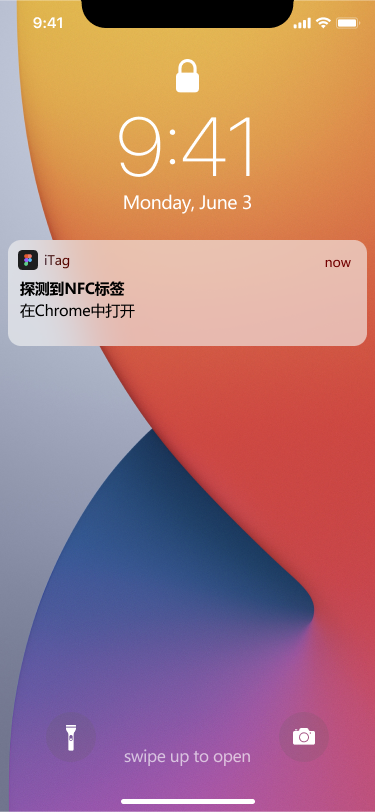
\includegraphics[scale=0.3]{iPhone11X.png}
        \end{minipage}
    }
    \subfigure[]
    {
        \begin{minipage}[b]{.3\linewidth}
            \centering
            
\includegraphics[scale=0.3]{Loggedout.png}
        \end{minipage}
    }
    \subfigure[]
    {
         \begin{minipage}[b]{.3\linewidth}
            \centering
            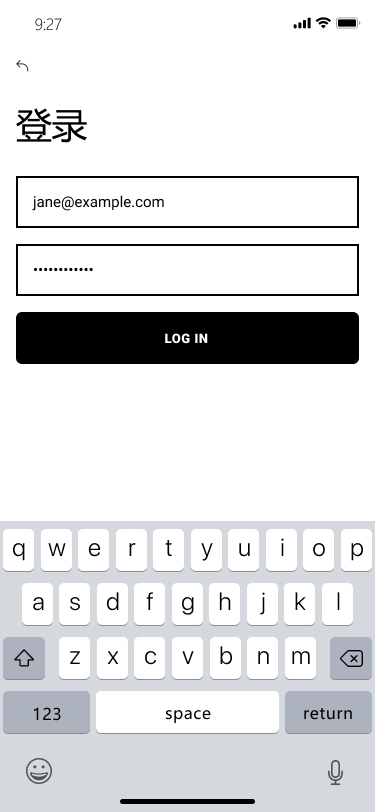
\includegraphics[scale=0.3]{Login.png}
        \end{minipage}
    }
    \caption{NFC扫描后登陆}
    \label{Login}
\end{figure}

注册新账号的时候会引导填写姓名和上传头像,为了降低用户的心理负担,可以选择不填写真名,并使用默认的预设图片,如图~\ref{Register}所示。

\begin{figure}[htbp]
    \centering
    \subfigure[]
    {
        \begin{minipage}[b]{.3\linewidth}
            \centering
            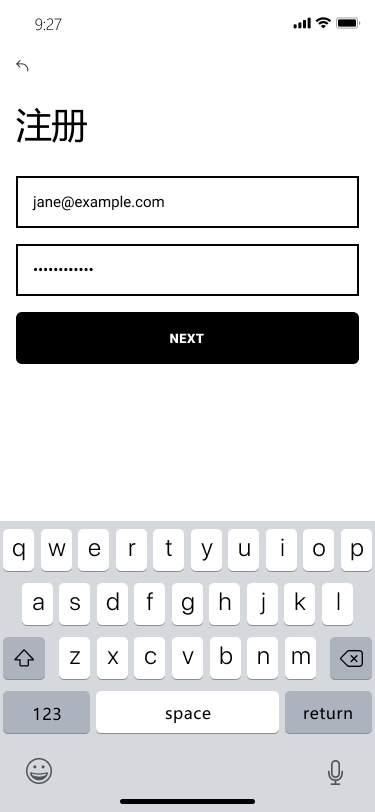
\includegraphics[scale=0.3]{Registerstep1.png}
        \end{minipage}
    }
    \subfigure[]
    {
         \begin{minipage}[b]{.3\linewidth}
            \centering
            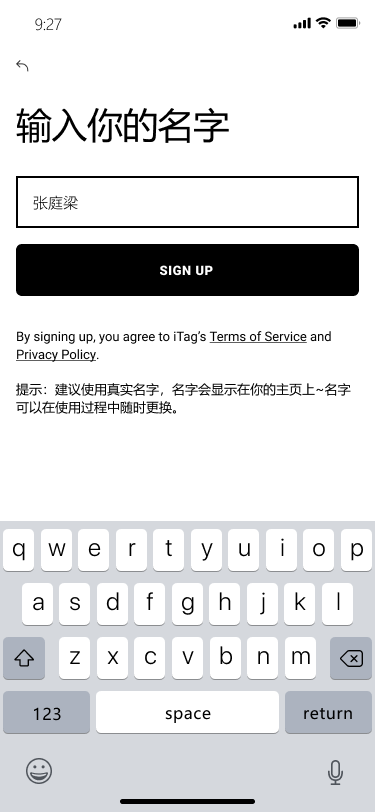
\includegraphics[scale=0.3]{Registerstep2.png}
        \end{minipage}
    }
    \subfigure[]
    {
         \begin{minipage}[b]{.3\linewidth}
            \centering
            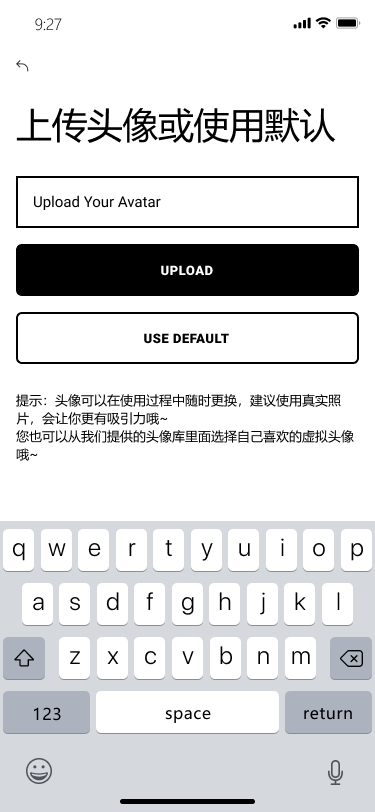
\includegraphics[scale=0.3]{Registerstep3.png}
        \end{minipage}
    }
    \caption{注册流程}
    \label{Register}
\end{figure}

完成后可以生成一个默认的预设界面,可以在这个基础上去添加信息。比如编辑主页背景等。最重要的其实是添加社交软件,可以选择多样的社交软件添加,有完备的import wizard帮助你傻瓜式添加社交账号预设,如图~\ref{EditHomepage}所示。

\begin{figure}[htbp]
    \centering
    \subfigure[]
    {
         \begin{minipage}[b]{.3\linewidth}
            \centering
            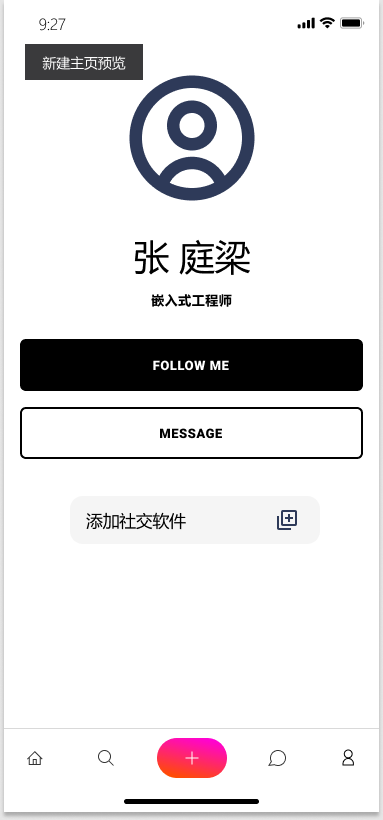
\includegraphics[scale=0.3]{NewHomePage.png}
        \end{minipage}
    }
    \subfigure[]
    {
        \begin{minipage}[b]{.3\linewidth}
            \centering
            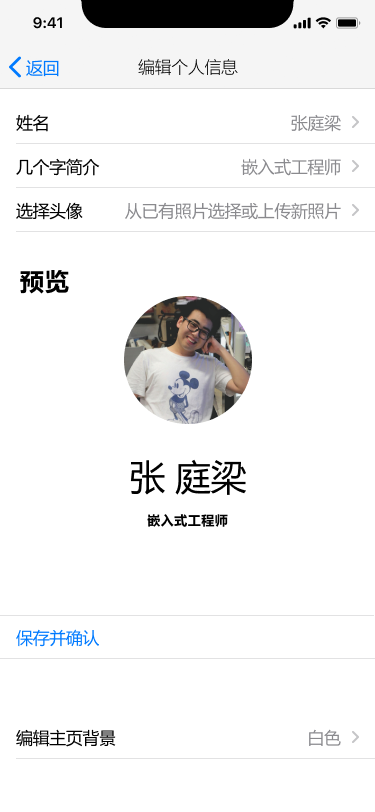
\includegraphics[scale=0.3]{EditHomepageProfile.png}
        \end{minipage}
    }
    \subfigure[]
    {
         \begin{minipage}[b]{.3\linewidth}
            \centering
            
\includegraphics[scale=0.3]{ChooseSocialAPP.png}
        \end{minipage}
    }
    \caption{编辑主页预设}
    \label{EditHomepage}
\end{figure}

一些主页预设样例如图~\ref{HomepageExample}所示,主页的预设自由度非常高,高级用户或者企业用户甚至可以编写更多功能的HTML+Javascript,部署到我们的系统中。

\begin{figure}[htbp]
    \centering
    \subfigure[]
    {
         \begin{minipage}[b]{.3\linewidth}
            \centering
            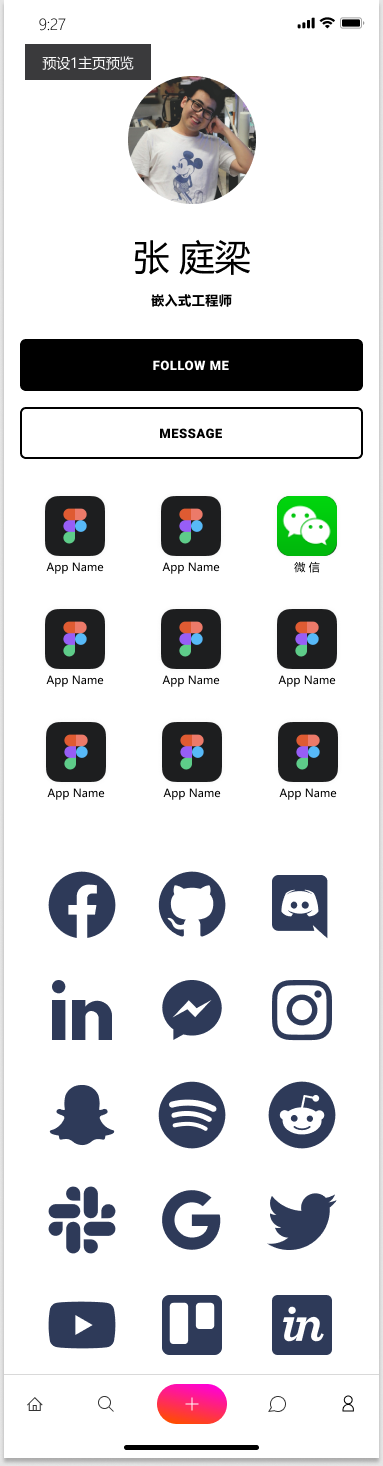
\includegraphics[scale=0.3]{EditHomePageofMyself.png}
        \end{minipage}
    }
    \subfigure[]
    {
        \begin{minipage}[b]{.3\linewidth}
            \centering
            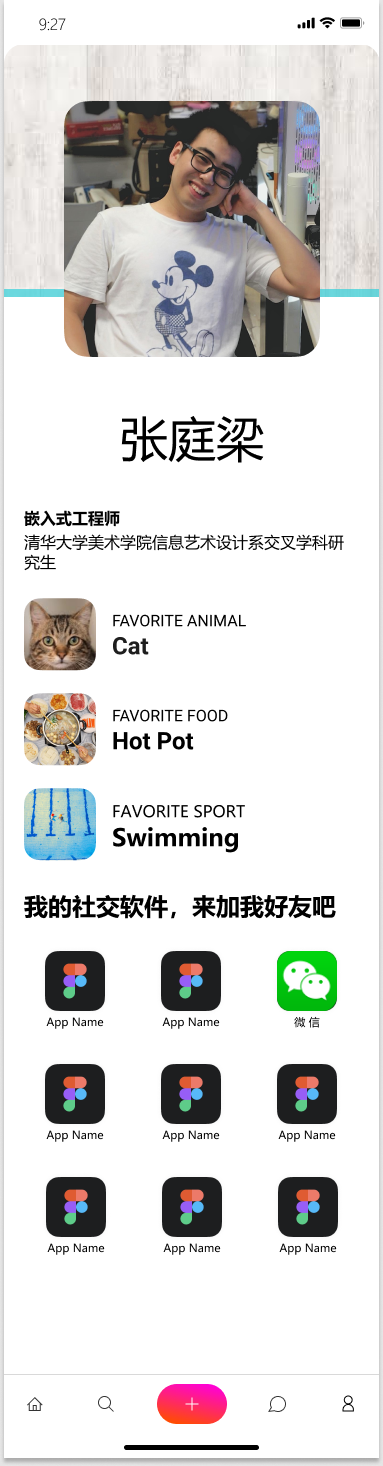
\includegraphics[scale=0.3]{HomePageofMyselfV0.png}
        \end{minipage}
    }
    \subfigure[]
    {
         \begin{minipage}[b]{.3\linewidth}
            \centering
            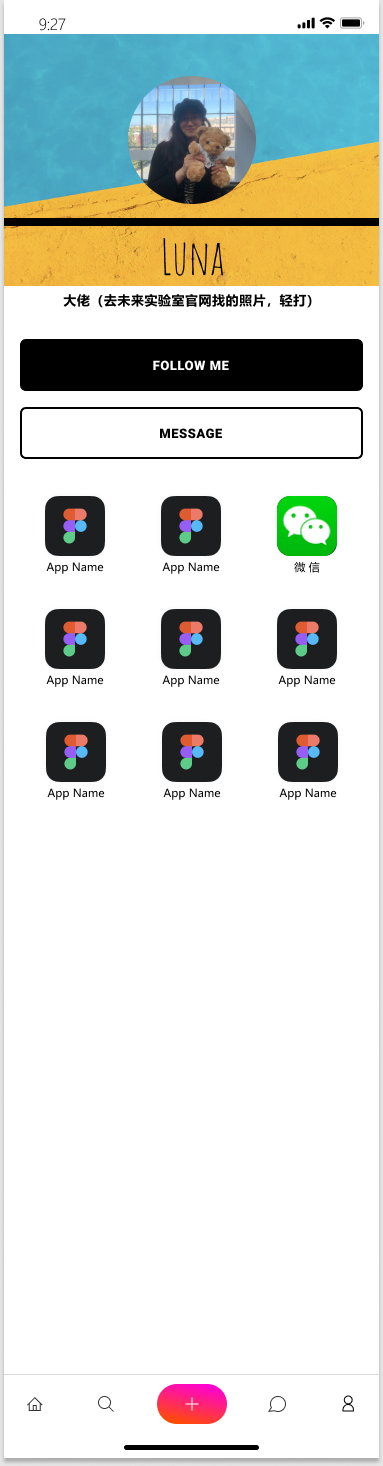
\includegraphics[scale=0.3]{ViewHomePage.png}
        \end{minipage}
    }
    \caption{主页预设样例}
    \label{HomepageExample}
\end{figure}

卡片管理系统也是保护个人隐私重要的一环,在这里你可以看到拥有的所有卡片,方便改变卡片显示的内容(即实现定义好的预设),同时可以设置权限,即特定的用户可见,如图~\ref{CardManageSystem}所示。如果卡片丢失,可以在卡片管理页面一键禁用此卡片,以保证个人信息安全。

\begin{figure}[htbp]
    \centering
    \subfigure[]
    {
         \begin{minipage}[b]{.3\linewidth}
            \centering
            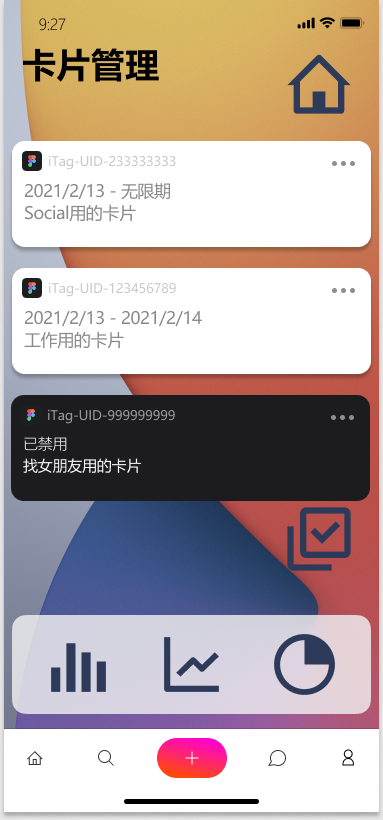
\includegraphics[scale=0.3]{NFCCardManageSystem.png}
        \end{minipage}
    }
    \subfigure[]
    {
        \begin{minipage}[b]{.3\linewidth}
            \centering
            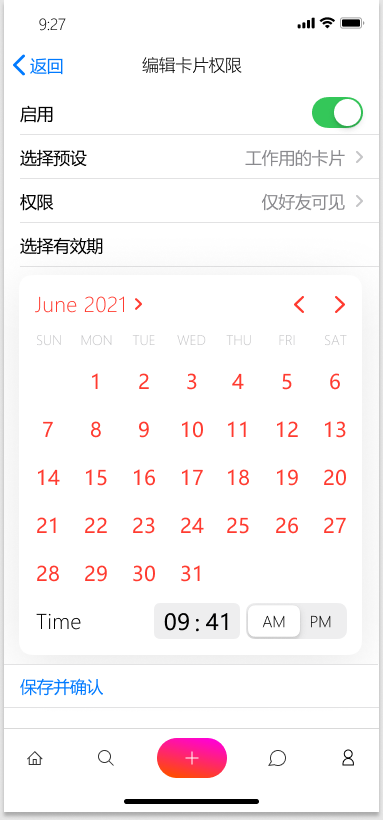
\includegraphics[scale=0.3]{NFCCardManage.png}
        \end{minipage}
    }
    \subfigure[]
    {
         \begin{minipage}[b]{.3\linewidth}
            \centering
            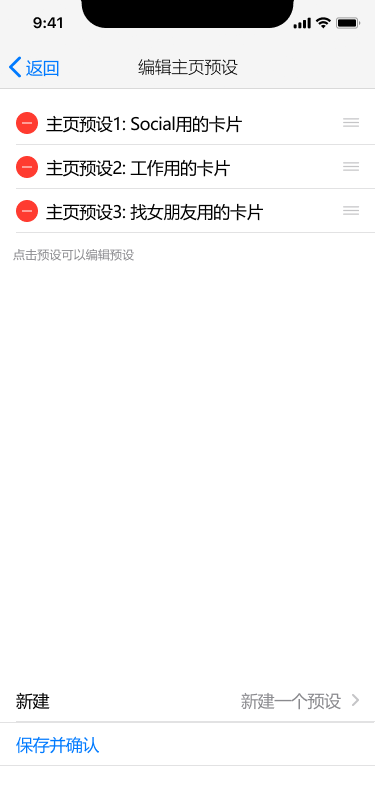
\includegraphics[scale=0.3]{EditHomepagePreset.png}
        \end{minipage}
    }
    \caption{卡片管理系统}
    \label{CardManageSystem}
\end{figure}

简单设置好预设后,这张卡片的链接会自动绑定到你选择的预设页面,当碰一碰其他人的手机时,对方的手机将会提示打开这一页面。微信比较特别,一般时通过扫描二维码或者搜索微信号添加好友,所以会有详尽的引导(保存图片-扫一扫添加)。其他软件如Github、Instagram、Bilibili等都有直链网址,直接打开即可,如图~\ref{ScanProcedure}所示。

\begin{figure}[htbp]
    \centering
    \subfigure[]
    {
         \begin{minipage}[b]{.3\linewidth}
            \centering
            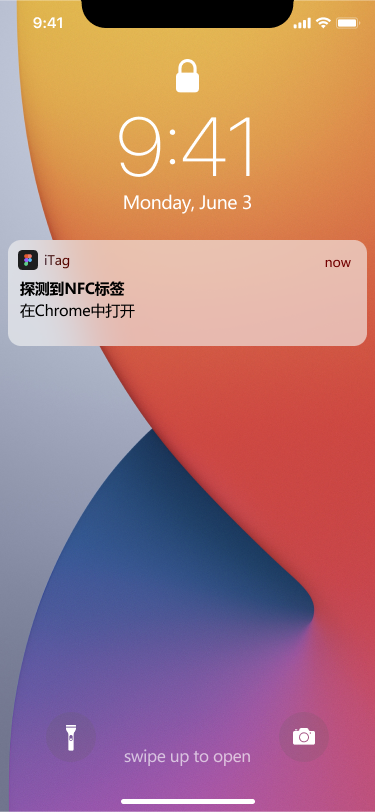
\includegraphics[scale=0.3]{iPhone11X.png}
        \end{minipage}
    }
    \subfigure[]
    {
        \begin{minipage}[b]{.3\linewidth}
            \centering
            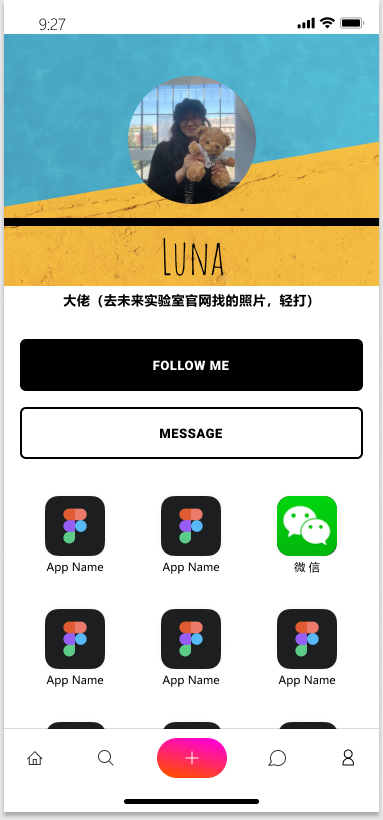
\includegraphics[scale=0.3]{ViewHomePageSmall.png}
        \end{minipage}
    }
    \subfigure[]
    {
         \begin{minipage}[b]{.3\linewidth}
            \centering
            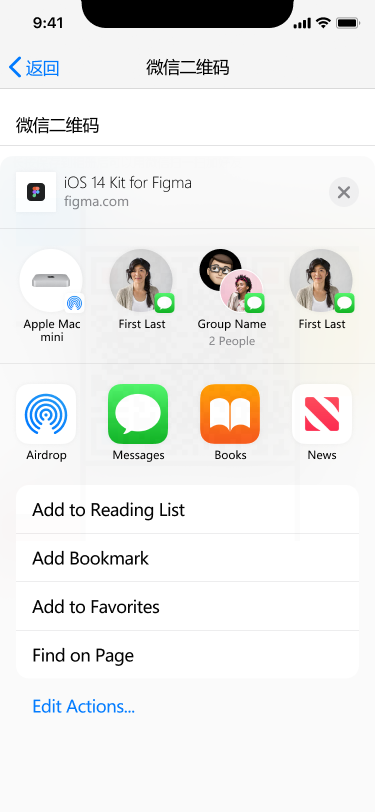
\includegraphics[scale=0.3]{ShareWechat.png}
        \end{minipage}
    }
    \caption{对方扫描流程}
    \label{ScanProcedure}
\end{figure}

在软件部分的最后我们重提隐私安全问题:

如前所述,几乎每一个流行的陌生人社交软件都曾被网络攻击,发生用户隐私数据被窃取或倒卖事件。由于陌生人社交信息数据量大而且敏感,一旦被窃取,可能会用于诈骗甚至可以分析出每个人的偏好,如果公开可能会对用户造成极大的影响,甚至造成社会性死亡。

所以在iTag设计之初我们就很重视用户的隐私安全:

由于我们不要求用户提供位置信息和其他的真实个人信息,用户的心理负担更小。

NFC卡片中只有一个带有SHA256加密后的UID信息,链接到特定的自定义页面中。同时NFC芯片也自带硬件加密,KeyAB一定程度上保证破解器很难读写卡内信息。对于特别关注信息安全的用户,我们还特别设计CPU卡版本,从硬件层面提供信息安全保证。

同时我们使用去中心化的区块链保存用户提供的部分个人信息,隐私信息能够被妥善保存。

\section{游戏策划}

一款类Ingress的基于地理位置的大型多人侵入式虚拟现实游戏。

\begin{tcolorbox}[breakable]
    游戏的故事背景是一群欧洲科学家偶然发现某种神秘的能量XM(Exotic Matter),这一能量的来源和用途无人知晓,研究人员认为可以开发并善用这能量,但另一方面却担心这样的能量会影响人们的思考甚至被能量本身奴役。

    游戏中有两大主要阵营,这两大互相争夺主控权的全球性组织分别是“反抗军”和“启蒙军”。“启蒙军”(Enlightened,以绿色标示)阵营希望能接纳这股“神秘的能量XM”,并相信这股能量能赐予人类进步与改革,其追随者相信神秘的能量会催生影响重大的“启蒙运动”,使全人类进化。另一派“反抗军”(Resistance,以蓝色标示)阵营则奋力捍卫并守护仅存的人性,有些人认为他们对于变化或进步感到畏惧,但反抗军坚信这一切都是为了保护人类。游戏的玩家被称为特工(Agent),两个阵营互相角力,争夺控制真实世界中的地标性建筑或雕塑等Portal(译作“传送门”)。

    游戏内容和真实世界的地理状况结合,游戏会透过手持装置的GPS、AGPS以及Wi-Fi信息确认玩家的位置,而玩家可以透过游戏的扫描器(Scanner)界面看到自身周围的传送门、XM或物品。游戏地图上各处散落着白色亮点,代表XM所在的位置,玩家在接近XM时会自动收集,而对传送门进行任何操作均需耗用XM。传送门主要是各种建筑、雕塑、艺术品等,玩家需亲自持手机接近这些传送门,进行部署(Deploy)、入侵(Hack)、补充能量(Recharge)、发射XMP等动作。玩家在游戏中的目标是透过连接多个本阵营控制的传送门,建立控制场(Control Field),覆盖最多的“Mind Units(MUs)”。

    在游戏中,全球各处存在着大量传送门(Portal),可以在游戏软件中察看。传送门都与实际地标关联,并且位在可被公众探访且步行能抵达的地点,例如:雕塑、壁画、公共艺术、喷泉、艺术涂鸦、图书馆、教学楼、水塔、邮局、纪念馆、宗教建筑、地铁站;醒目的建筑和独特的当地企业;国家公园、露营地、主题公园的入口等。根据当前控制传送门的阵营不同,传送门会呈现出不同的颜色:启蒙军阵营控制时为绿色,反抗军阵营控制时为蓝色,无人控制时为灰色,双方的玩家都可以占领这些灰色的传送门。

    游戏的目的是争夺传送门并制造控制场(Control Field),以获取Mind Units。玩家可以使用炸弹(XMP)攻击敌方传送门,削弱目标据点共振器的能量值,要是一个共振器失去全部能量,它就被摧毁了。如果全部的共振器都被摧毁,传送门就会转为中性(Neutral),玩家接着可以放置最多八个共振器控制该传送门。另外,共振器的能量每天都会下降,而玩家可以替他充能(Recharge)以使其保持较高的能量,以免敌人轻易摧毁这些共振器。除了在传送门旁边直接替它充能,玩家若持有一条传送门的钥匙亦可在一定距离外替它充能,只是充能效益(Recharge Efficiency)会随玩家与传送门的距离有所衰减。

    当两个传送门都已摆满八个共振器,而玩家同时持有目标的钥匙、目标在所在传送门的覆盖范围之内、不在任何一个Field(该Portal作为顶点的情况除外)内、路径内没有其他的Link这几个条件全部达成,就可以在两个传送门间建立链接(Link)。如果玩家在游戏中使三个传送门连成三角形,就会产生一个控制场(Control Field)。控制场会让玩家的阵营获得Mind Units(MUs),MUs的数量与Field所覆盖范围的人口密度与Field大小有关,玩家在局势 (Intel)标签下可以查看两大阵营各自累积了多少MUs。

    当Portal因为被攻击/能量丧失等原因导致剩下3个以及3个以下的Resonator时,该Portal所连接的所有Link将会失效,同时以其为顶点的Field也会失效。且有几率掉落向外连接的Link的目标的Portal Key。

    由于三角形潜在的相互嵌套的几何性质,玩家可依照特定的连结顺序,建立多重控制场 ,在同一区域获取多倍的 AP 值。 玩家也能够利用情报地图(Intel Map)查看区域乃至世界的连结及控制场布局,规划战略。\cite{wiki:Ingress}
\end{tcolorbox}


未来我们官方及其社群为了加强玩家互动,会不定期组织一系列官方、半官方特别活动,以调动玩家的积极性。如图~\ref{Ingress}所示。

\begin{figure}[htbp]
    \centering
    \subfigure[]
    {
         \begin{minipage}[b]{.3\linewidth}
            \centering
            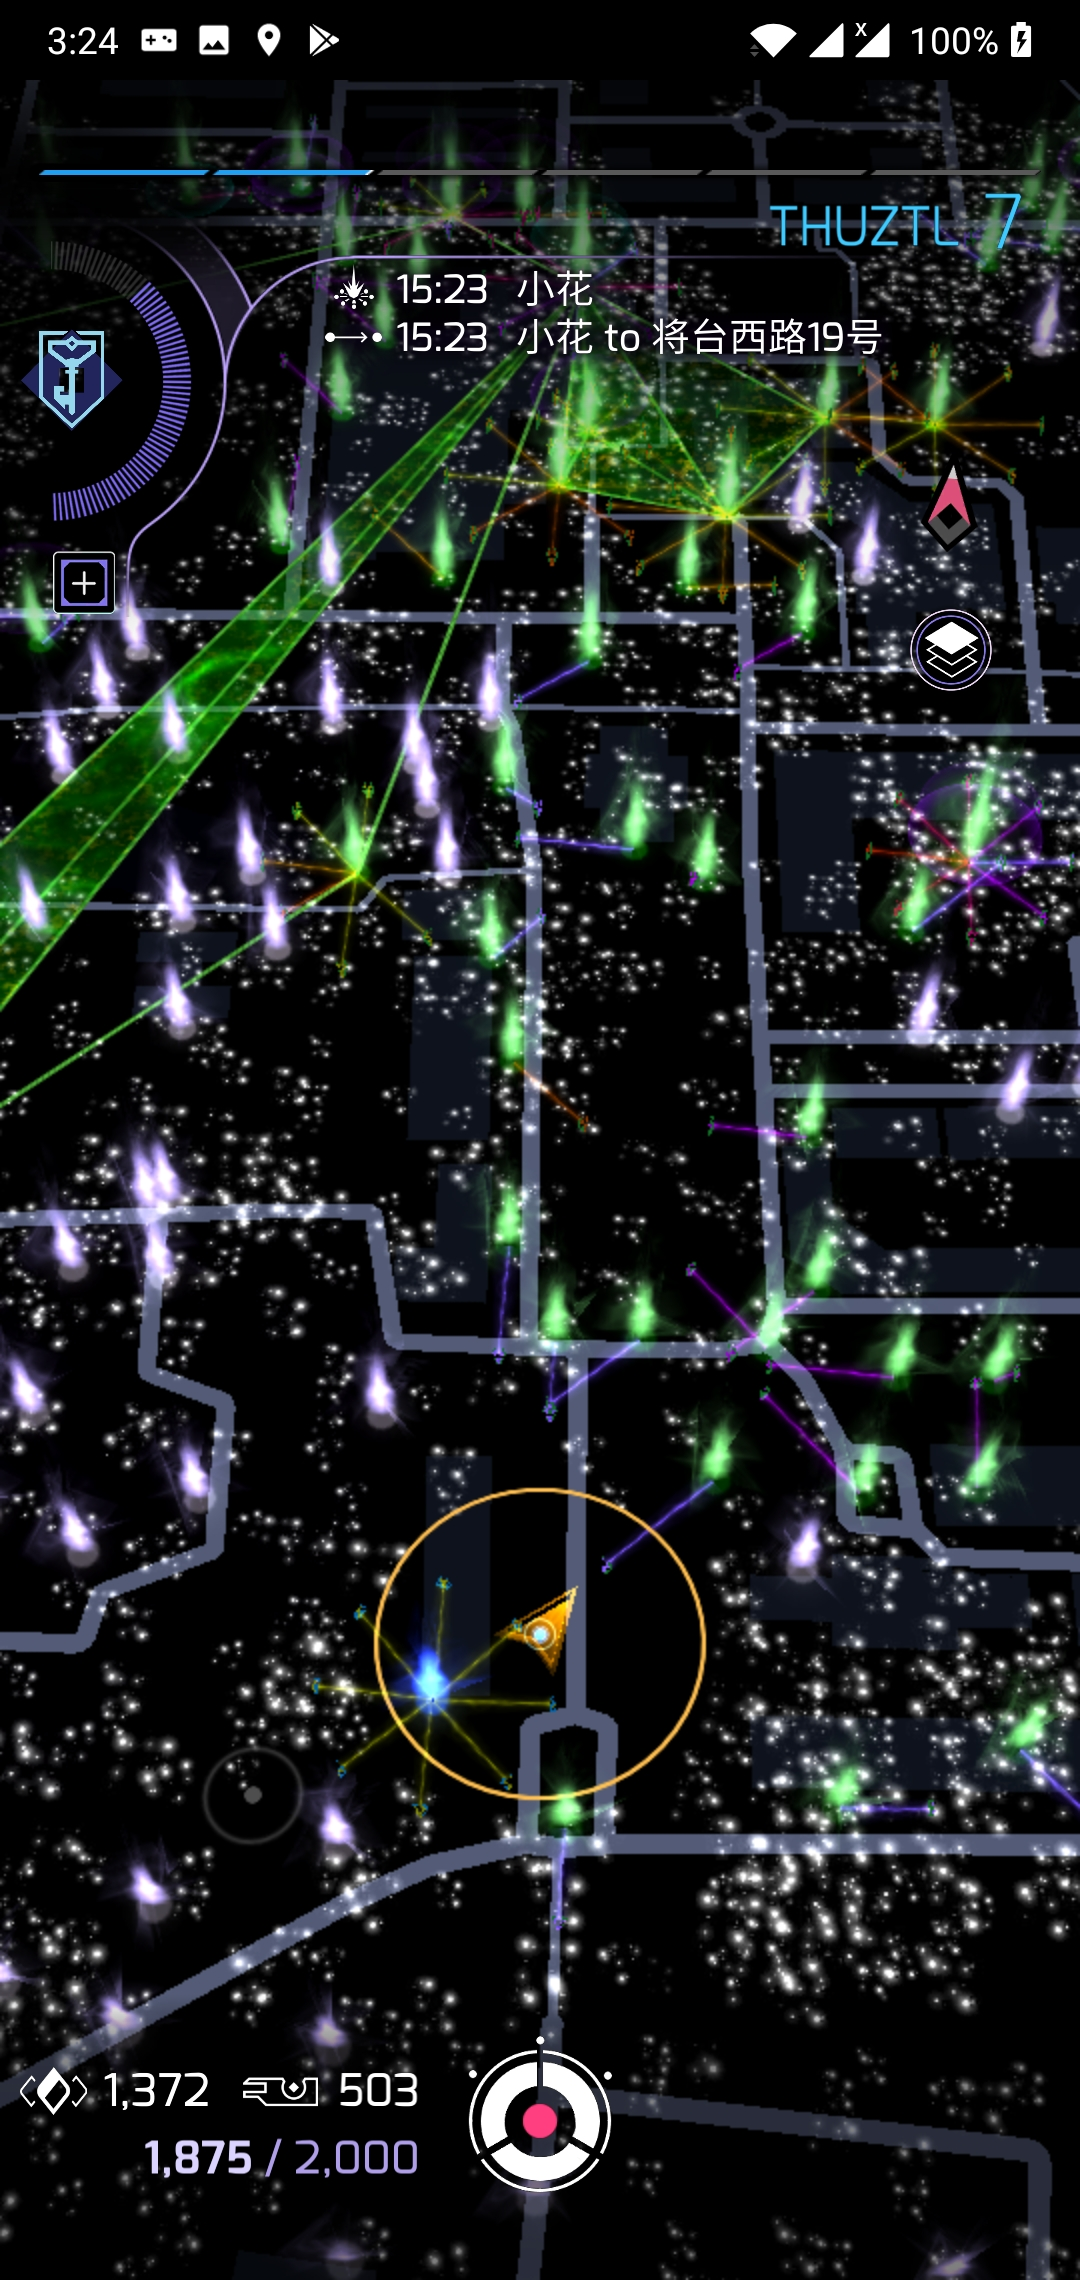
\includegraphics[scale=0.1]{Ingress0.jpg}
        \end{minipage}
    }
    \subfigure[]
    {
        \begin{minipage}[b]{.3\linewidth}
            \centering
            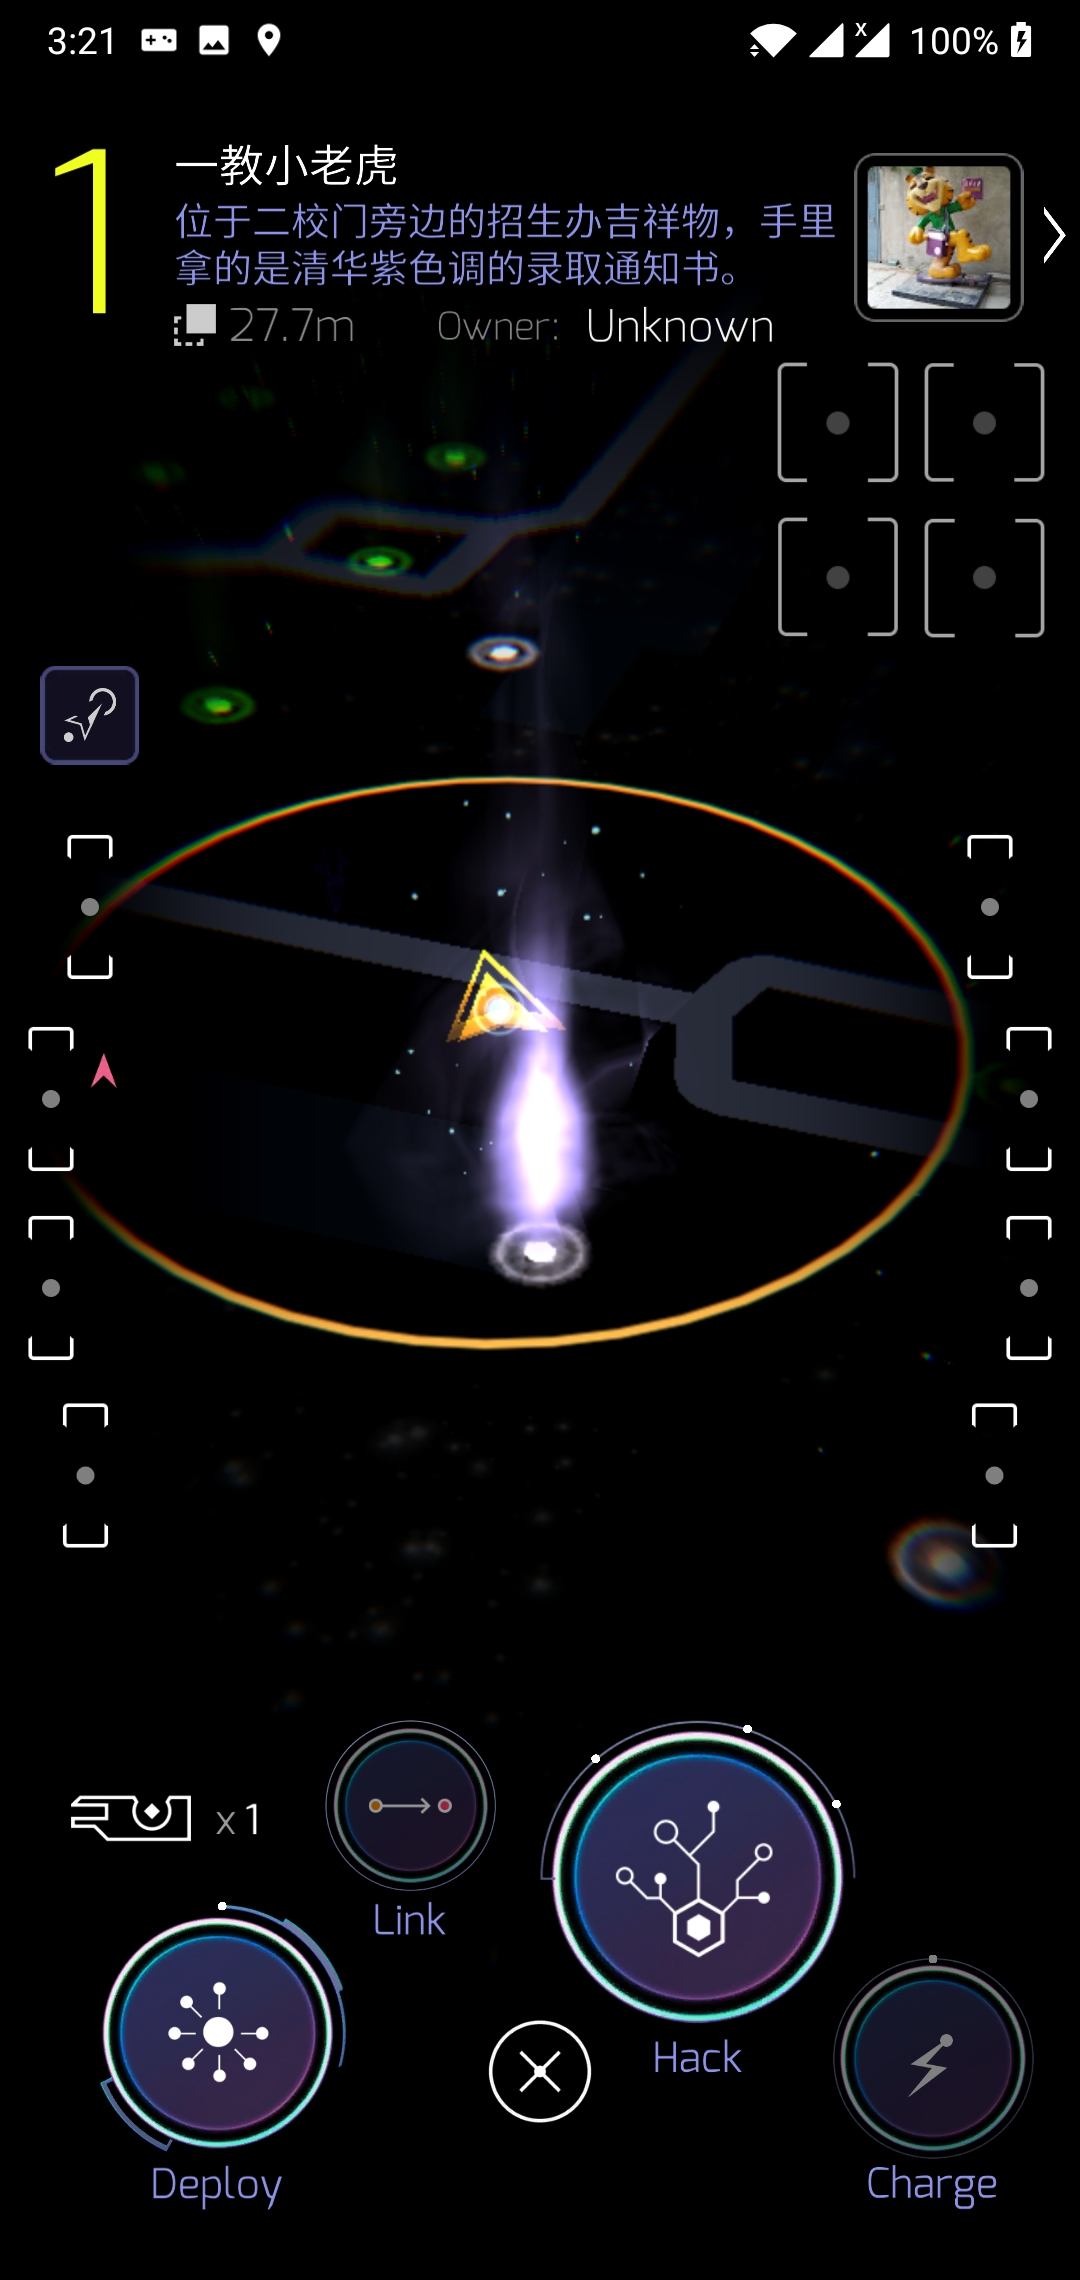
\includegraphics[scale=0.1]{Ingress1.jpg}
        \end{minipage}
    }
    \subfigure[]
    {
         \begin{minipage}[b]{.3\linewidth}
            \centering
            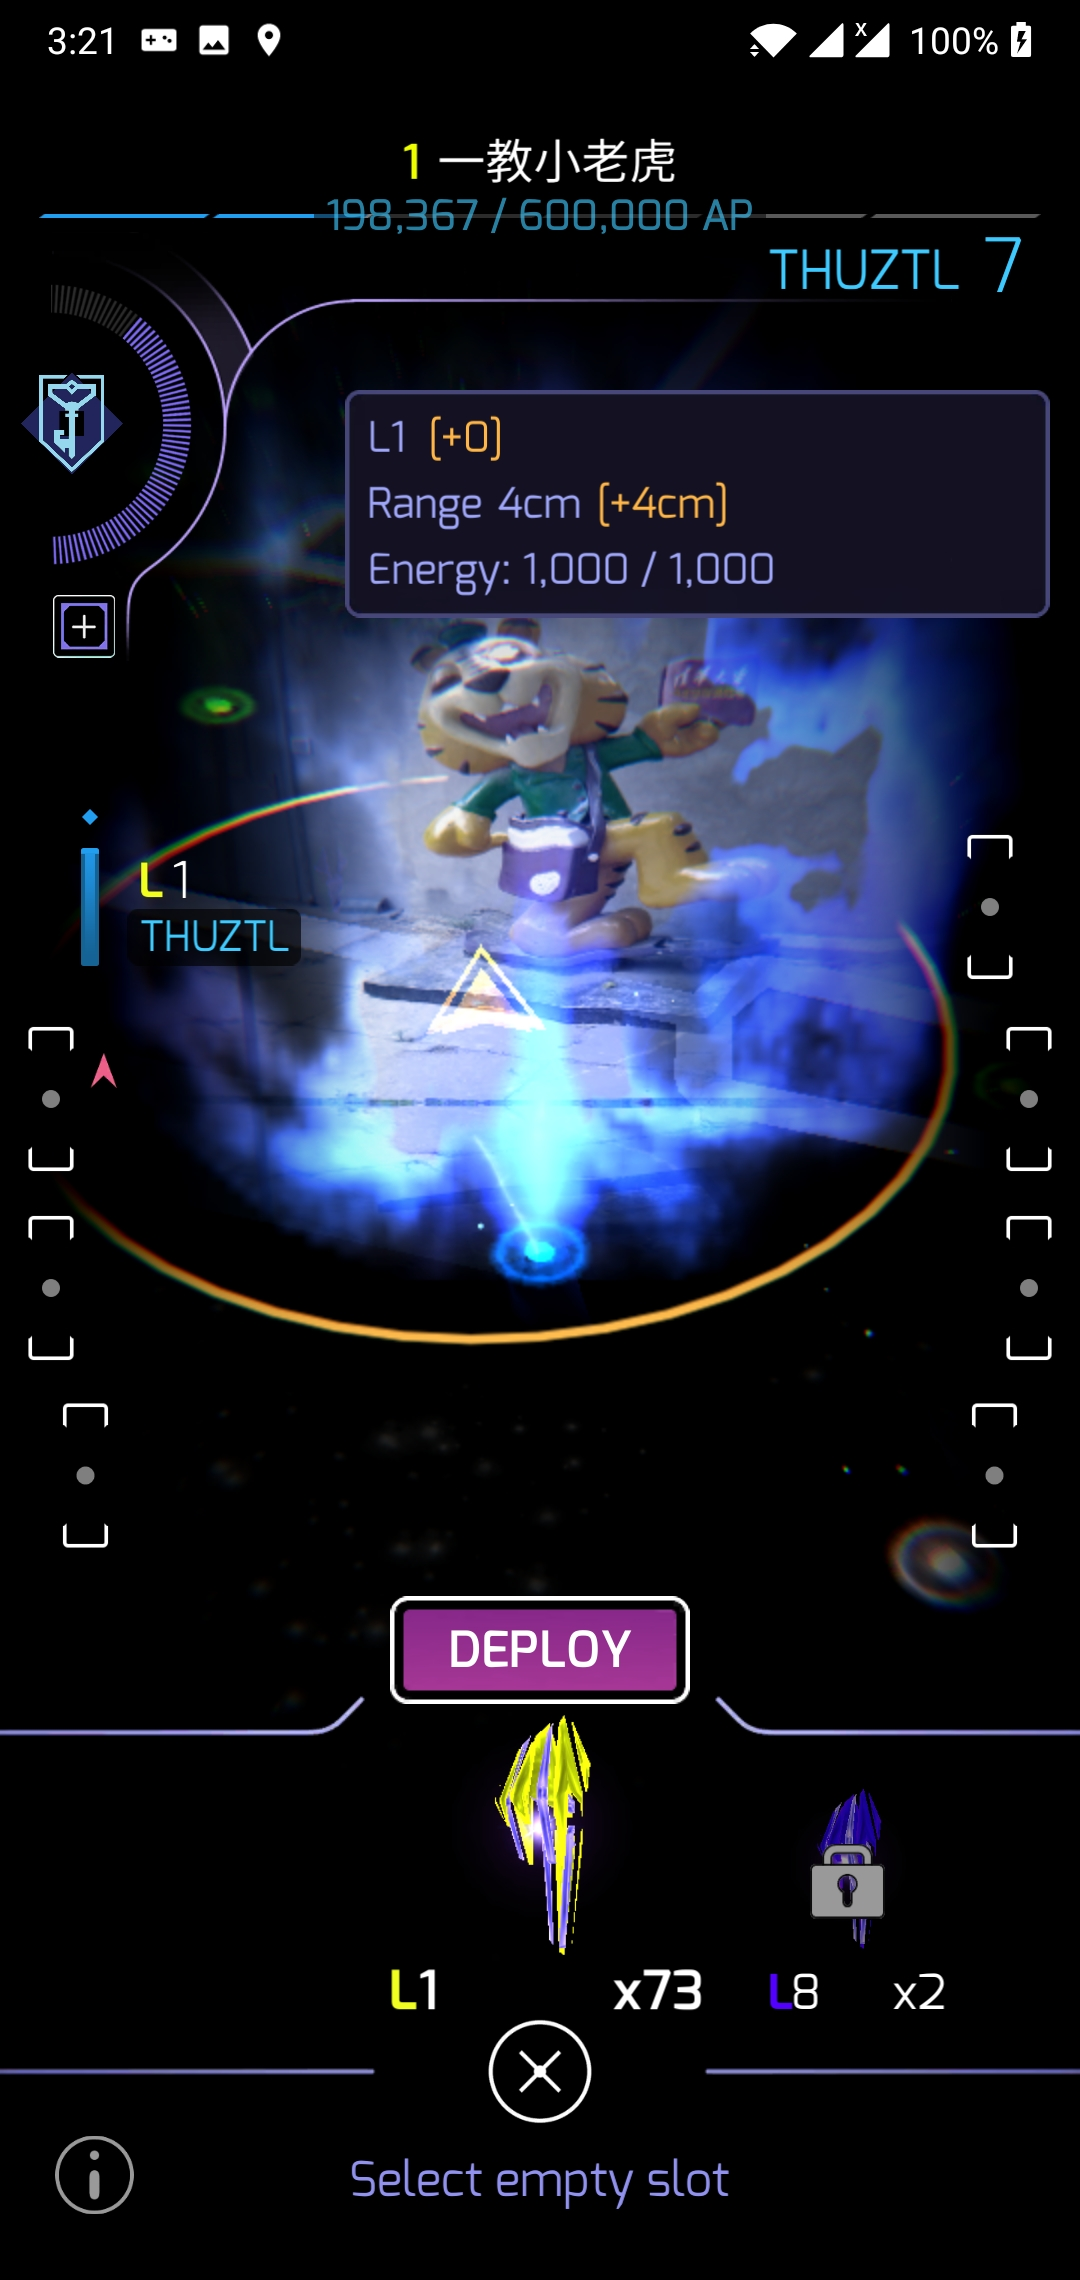
\includegraphics[scale=0.1]{Ingress2.jpg}
        \end{minipage}
    }
    \caption{游戏机制示意}
    \label{Ingress}
\end{figure}

在定位技术细节方面,高德地图或Google Maps的授权费用过高,我们选择使用OpenStreetMap地图源。而且Google Maps在中国大陆境内不能正确显示地理位置,其原因为中国大陆以国家安全为由要求所有境内地图测绘单位使用国家自行定制的GCJ-02 坐标系统,该系统对GPS使用的WGS84坐标系统进行偏移,所以其地图与实际坐标有500米左右的偏移。而由于GPS坐标系统与OSM坐标系统使用的卫星坐标体系一致,因此坐标偏移问题得以解决。

\section{盈利模式}

内测阶段基本不盈利,运营成本由Kickstarter等众筹平台和内测版本iTag卡片出售盈利以及捐赠款支持。由于初期服务器使用单个本地服务器和低性能阿里云服务器结合的方式,iTag使用国产NFC tag半成品生产,成本约几毛钱一个,可以实现盈亏相抵。

用户量破万后,主要是联名款、定制款和智能款iTag出售盈利。

用户百万量级时(游戏系统上线),游戏内购可以作为一部分盈利来源,同时,引入赞助,赞助商家可以将门店设置为portal所在地,从而吸引玩家前来朝圣或聚集。比如餐厅、咖啡店、超市等,可以通过这一方式吸引顾客特别是游客。相当于一种隐性的广告。

经过慎重考虑,我们决定软件本体永久免费,而且社交主页永久没有广告,给用户做出这一承诺有助于吸引更多的用户。

在用户接近千万时,说明软件热度已经达到一个里程碑,我们将进一步发行游戏周边,以及联名款卡片。

\section{参考文献}

\bibliography{social}
\bibliographystyle{plain}

\newpage
\section{附录}

\begin{figure}[htbp]
    \centering
    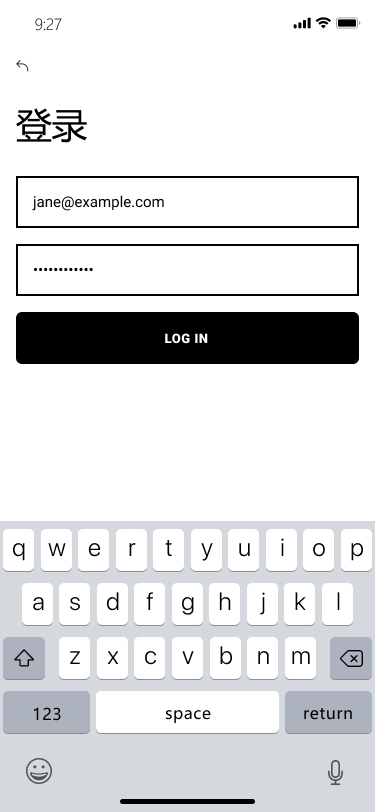
\includegraphics[width=\linewidth]{Login.png}
    \caption{嘿嘿嘿} 
    \label{1}
\end{figure}

\end{document}